\documentclass[conf]{new-aiaa}
%\documentclass[journal]{new-aiaa} %for journal papers
%\documentclass[a4paper]{article}
%\documentclass{homework}

%% Sets page size and margins
%\usepackage[a4paper,top=3cm,bottom=2cm,left=3cm,right=3cm,marginparwidth=0.8.75cm]{geometry}

%\usepackage[utf8]{inputenc}
\usepackage{graphicx}
\usepackage{amsmath}
\usepackage[version=4]{mhchem}
\usepackage{siunitx}
\usepackage{longtable,tabularx}
\setlength\LTleft{0pt} 
%======================================

% additions
\graphicspath{ {figures/} }
\usepackage{floatrow}
\usepackage{ar}
\usepackage{amstext} % for \text macro
\usepackage{array}   % for \newcolumntype macro
\usepackage{gensymb} % for degree symbol
\newcolumntype{L}{>{$}l<{$}} % math-mode version of "l" column type
\usepackage[numbered,framed]{matlab-prettifier}
\usepackage{fancyvrb}

\pagestyle{empty}

\definecolor{listinggray}{gray}{0.9}
\definecolor{lbcolor}{rgb}{0.9,0.9,0.9}
\lstset{
backgroundcolor=\color{lbcolor},
    tabsize=4,    
%   rulecolor=,
    language=fortran,
        basicstyle=\mlttfamily,
        upquote=true,
        aboveskip={1.5\baselineskip},
        columns=fixed,
        showstringspaces=false,
        extendedchars=false,
        breaklines=true,
        prebreak = \raisebox{0ex}[0ex][0ex]{\ensuremath{\hookleftarrow}},
        frame=single,
        numbers=left,
        showtabs=false,
        showspaces=false,
        showstringspaces=false,
        identifierstyle=\mlttfamily,
				keywordstyle=\color{blue}\mlttfamily,
				stringstyle=\color{red}\mlttfamily,
				commentstyle=\color[RGB]{34,139,34}\mlttfamily,
				morecomment=[l][\color{magenta}]{\#}
        %keywordstyle=\color[rgb]{0,0,1},
        %commentstyle=\color[rgb]{0.026,0.112,0.095},
        %stringstyle=\color[rgb]{0.627,0.126,0.941},
        %numberstyle=\color[rgb]{0.205, 0.142, 0.73},
%        \lstdefinestyle{C++}{language=C++,style=numbers}’.
}
%\usepackage{titlesec}
%\titleformat*{\paragraph}{\large\bfseries}
%======================================
\title{CE 791 HPC - Mini Project\\2D Groundwater Flow with FD}

\author{Andrew Navratil}

\begin{document}

\maketitle

The 2D groundwater flow equation is coded in Fortran using finite differences.  The forward Euler method is utilized for time stepping, using the provided finite difference approximation formula.  The delta x and delta y values are kept separate and allowed to differ.  The time step value utilized is 0.001 days after experimenting with various values (no stability analysis was performed on the equation to get a CFL number).  The transmissivity function coefficients are calculated using Matlab code with the conditions provided, giving values of a = -0.001, b = -0.002, c = 0.000004, and d = 2.0.  The boundary conditions are implemented as given, with homogeneous Neumann on the top and bottom, and nonhomogeneous Dirichlet on the left and right.

Parallelization is performed in MPI using 1D domain decomposition.  The 2D physical domain is partitioned into 1D blocks of columns, where the number of interior column nodes is specified to be divisible by all numbers of processors utilized, resulting in nx = 16*64, splitting the 1000m length.  A derived datatype for columns is created to enable passing ghost columns to left and right neighbor processors when calling MPI\_SENDRECV.  The multidimensional array storing the solution is purposely organized so that columns of the physical x-y domain are also columns in the solution i-j multidimensional array, and the derived type utilizes MPI\_TYPE\_CONTIGUOUS.  A virtual topology is created using MPI\_CART\_CREATE.

Performance plots are generated with Matlab, and the program is executed on henry2.  The execution time and mflops calculations are executed in Fortran for each run combo of num procs (1,2,4,8,16) and overall time (10, 100, 1000 days).  The values are printed to gw.out and manually copied into Matlab code for plotting.  The number of operations per grid point per iteration is estimated at 33 for the FDA.

Solution plots are also generated with Matlab for each of the three overall times.  The Fortran code writes out the solution to a txt file which is then imported into Matlab and plotted using contours.  The execution using 16 processors was utilized for producing the output data, with the additional goal of confirming the parallelization code.

\begin{figure}[H]
	\centering
	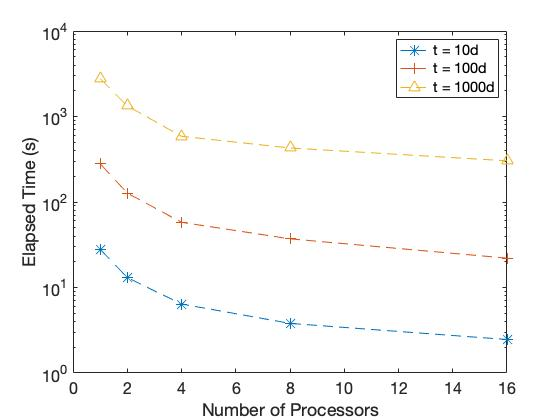
\includegraphics[width=1\columnwidth]{../miniplots/mini_times.jpg}
	\caption{Execution Times}
\end{figure}

The plot of execution times is done with a semi-log plot, with a log y-axis, in order to combine all three number of days together.  The expected trend is observed for a properly parallelized code, where execution time decreases as number of processors increases, and overall execution time increases as the number of days increases, using the same time step to ensure stability since the grid is the same.

\newpage

\begin{figure}[H]
	\centering
	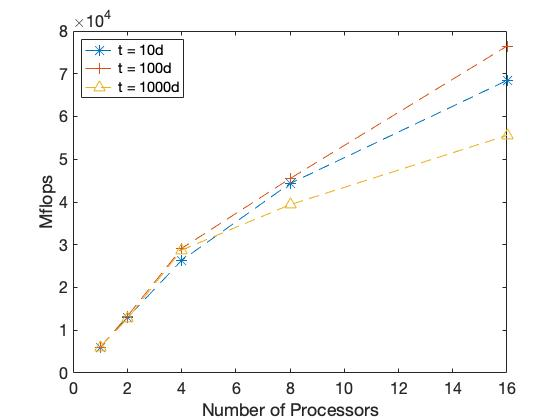
\includegraphics[width=1\columnwidth]{../miniplots/mini_mflops.jpg}
	\caption{Mflops}
\end{figure}

The plot of Mflops also shows the expected trend for a properly parallelized code.  The Mflops increases as the number of processors is increased, and this increase is at almost the same rate regardless of the amount of time it is run (both total number of ops and total execution times increase giving similar ratios for Mflops).  The performace does start to diverge around 8 processors, with an increase for 100 days and decrease for 1000 days.  The maximum performance seen at 16 processors is around 75 Gflops.

\newpage

\begin{figure}[H]
	\centering
	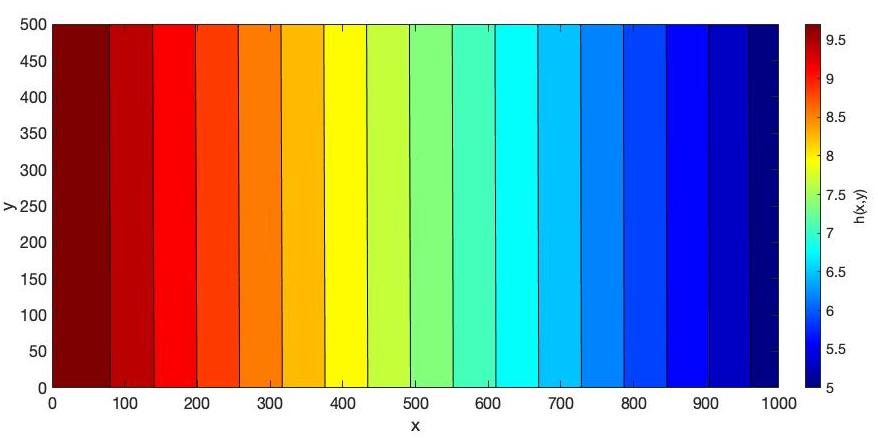
\includegraphics[width=1\columnwidth]{../miniplots/sln_0010.jpg}
	\caption{Solution at 10 days}
\end{figure}

\begin{figure}[H]
	\centering
	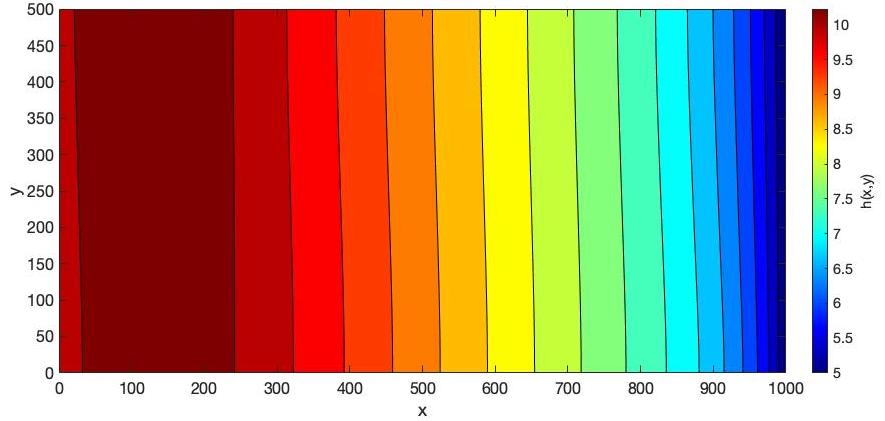
\includegraphics[width=1\columnwidth]{../miniplots/sln_0100.jpg}
	\caption{Solution at 100 days}
\end{figure}

\begin{figure}[H]
	\centering
	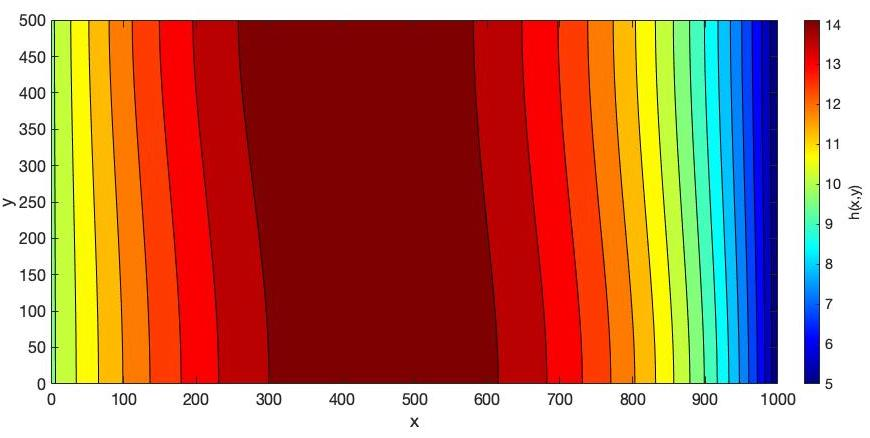
\includegraphics[width=1\columnwidth]{../miniplots/sln_1000.jpg}
	\caption{Solution at 1000 days}
\end{figure}

Solution plots are shown above.  We can see the left and right boundary conditions limiting the head values on the ends to 10m on the left end and 5m on the right end, for all number of days.  The uniform recharge varies in time and eventually causes the head to climb greater than the original maximum, reaching a maximum of 14.68m towards the left middle of the domain after 1000 days.  The bends in the contour lines showing a variation from bottom to top for the left to right gradient is due to the transmissivity function.

%======================================
\newpage

\section*{Fortran Code}
\lstinputlisting[language=fortran]{../gw.f90}

\newpage

\section*{Matlab Code}

\lstset{
  style      = Matlab-editor,
  basicstyle = \mlttfamily,
}
\lstinputlisting{../mini.m}

\newpage

\section*{gwout.txt}
\VerbatimInput{../miniplots/gwout.txt}

\end{document}



